\chapter{System Model}\label{ch:SystemModel}
\section{Background}
\section{Mathematical model of VSR}
The voltage equations for the 3-phase system shown in [\ref{fig:topology}] can be written as:
\begin{equation}
\begin{gathered}
    e_{a} = L \frac{di_a}{dt} + R i_a + \mathcal{V}_a\\
    e_{b} = L \frac{di_b}{dt} + R i_b + \mathcal{V}_b\\
    e_{c} = L \frac{di_c}{dt} + R i_c + \mathcal{V}_c
\end{gathered}
\label{eq:voltage_eq}
\end{equation}
where $e_{a}, e_{b}, e_{c}$ are the grid phase voltages, $i_a, i_b, i_c$ are the phase currents, $L$ is the input inductance,
$R$ is the input resistance, $\mathcal{V}_a, \mathcal{V}_b, \mathcal{V}_c$ are the rectifier terminal phase voltages.\par
The terminal voltages are determined by the modulation strategy, the DC link voltage and common mode voltage.\par
\begin{equation}
    \begin{gathered}
        \mathcal{V}_a = S_a V_{dc} + V_{cm}\\
        \mathcal{V}_b = S_b V_{dc} + V_{cm}\\
        \mathcal{V}_c = S_c V_{dc} + V_{cm}
    \end{gathered}
\label{eq:common_mode_voltage}
\end{equation}
where $S_a, S_b, S_c$ are the switching states of the converter switches, $V_{dc}$ is the DC link voltage and
$V_{cm}$ is the common mode voltage.\par
The common mode voltage can be calculated by adding the three phase voltages in equation[\ref{eq:voltage_eq}]
and the current equations for the three-phase system, $i_a + i_b + i_c = 0$, which leads to the following
equation:
\begin{equation}
    \begin{gathered}
        V_{cm} =\frac{1}{3}(e_a + e_b + e_c) -\frac{1}{3}(S_a + S_b + S_c) V_{dc}\\
    \end{gathered}
    \label{eq:common_mode_voltage_calc}
\end{equation}
\section{Symmetrical sequence decomposition}
Incase of unbalanced grid conditions, the symmetrical sequence decomposition is used to analyze
the system as shown in figure[\ref{fig:symmetricalDecomposition}]. The three-phase parameters can
be decomposed into positive, negative, and zero sequence components represented by equation[\ref{eq:symmetrical_component}].
Since the neutral point of the system is not connected to the ground, the zero sequence component is not present in the system.
The derivation and Implementation of the symmetrical sequence decomposition is given in appendix \ref{App:SymmetricalComponents}.
\begin{equation}
    \begin{gathered}
        X_{abc} = X^{p}_{abc} + X^{n}_{abc} + X^{0}_{abc}
    \end{gathered}
    \label{eq:symmetrical_component}
\end{equation}
where $X_{abc}$ is the three-phase parameter, $X^{p}_{abc}, X^{n}_{abc}, X^{0}_{abc}$ are the positive, negative,
and zero sequence components respectively.\par
Thus the space vector of the unbalanced system can be transformed using the Clarke transformation as given in appendix \ref{App:ClarkParkTransformation}
to $\alpha\beta$ coordinates as space vector sum of the positive $X_{\alpha\beta}$ and negative $X_{\alpha\beta}$ sequence components.
The model of the system in equation[\ref{eq:alpha_beta_model}] can be expressed in $\alpha\beta$ coordinates as follows:\par
\begin{equation}
    \begin{split}
            e^{p}_{\alpha} &=  L  \frac{d}{dt} i^{p}_{\alpha} + R i^{p}_{\alpha} + \mathcal{V}^{p}_{\alpha} \\
            e^{p}_{\beta} &=  L  \frac{d}{dt} i^{p}_{\beta} + R i^{p}_{\beta} + \mathcal{V}^{p}_{\beta} \\
            e^{n}_{\alpha} &=  L  \frac{d}{dt} i^{n}_{\alpha} + R i^{n}_{\alpha} + \mathcal{V}^{n}_{\alpha} \\
            e^{n}_{\beta} &=  L  \frac{d}{dt} i^{n}_{\beta} + R i^{n}_{\beta} + \mathcal{V}^{n}_{\beta} 
    \end{split}
    \label{eq:alpha_beta_model}
\end{equation}
\begin{figure}[H]
    \centering
    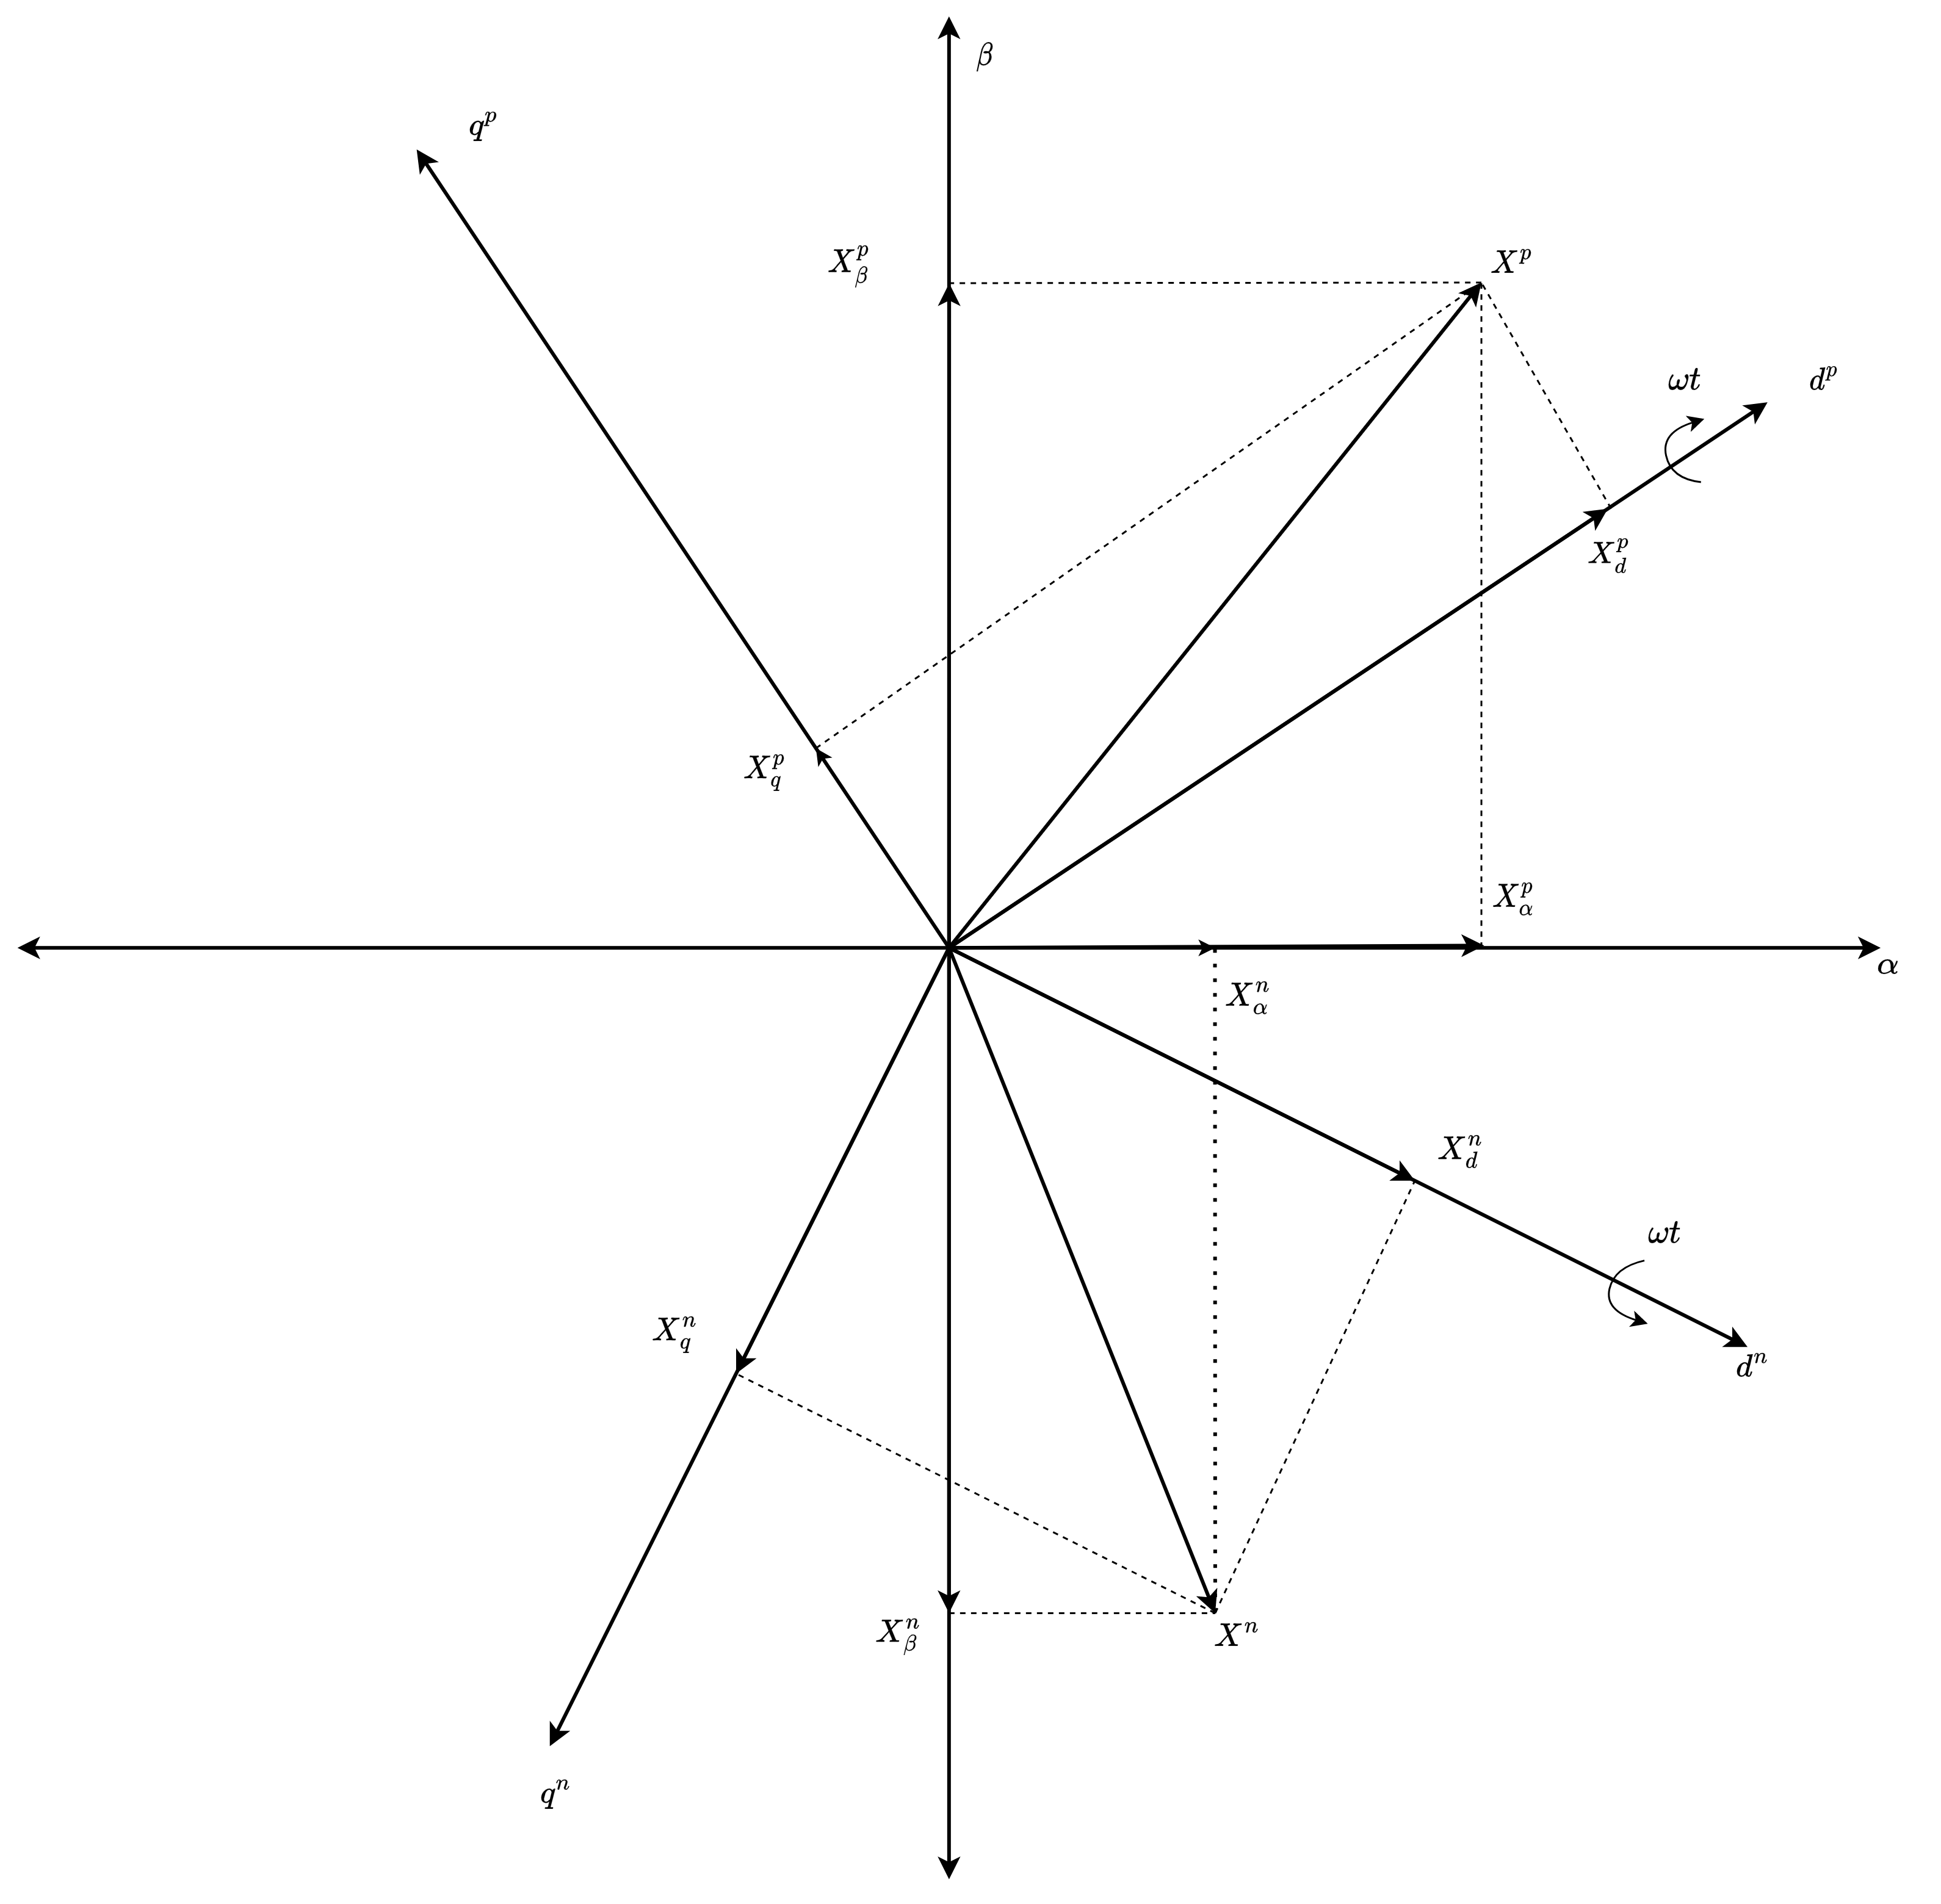
\includegraphics[scale=0.35]{img/symmetricalDecomposition.png}
    \caption{Phasor representation of unbalanced three-phase system}
    \label{fig:symmetricalDecomposition}
\end{figure}
The mathematical model of the system can be expressed in state space form in $\alpha\beta$ coordinates as follows
\begin{equation}
    \begin{split}
        \frac{d}{dt}
        \begin{bmatrix}
            i^{p}_{\alpha} \\
            i^{p}_{\beta}
        \end{bmatrix}
        =
        \begin{bmatrix}
            -\frac{R}{L} & 0 \\
            0 & -\frac{R}{L}
        \end{bmatrix}
        \begin{bmatrix}
            i^{p}_{\alpha} \\
            i^{p}_{\beta}
        \end{bmatrix}
        +
        \begin{bmatrix}
            \frac{1}{L} & 0 \\
            0 & \frac{1}{L}
        \end{bmatrix}
        \begin{bmatrix}
            e^{p}_{\alpha} \\
            e^{p}_{\beta}
        \end{bmatrix}
        +
        \begin{bmatrix}
            -\frac{1}{L} & 0 \\
            0 & -\frac{1}{L}
        \end{bmatrix}
        \begin{bmatrix}
            \mathcal{V}^{p}_{\alpha} \\
            \mathcal{V}^{p}_{\beta}
        \end{bmatrix}
\end{split}
    \label{eq:state_space_alpha_beta_positive}
\end{equation}
\begin{equation}
    \begin{split}
        \frac{d}{dt}
        \begin{bmatrix}
            i^{n}_{\alpha} \\
            i^{n}_{\beta}
        \end{bmatrix}
        =
        \begin{bmatrix}
            -\frac{R}{L} & 0 \\
            0 & -\frac{R}{L}
        \end{bmatrix}
        \begin{bmatrix}
            i^{n}_{\alpha} \\
            i^{n}_{\beta}
        \end{bmatrix}
        +
        \begin{bmatrix}
            \frac{1}{L} & 0 \\
            0 & \frac{1}{L}
        \end{bmatrix}
        \begin{bmatrix}
            e^{n}_{\alpha} \\
            e^{n}_{\beta}
        \end{bmatrix}
        +
        \begin{bmatrix}
            -\frac{1}{L} & 0 \\
            0 & -\frac{1}{L}
        \end{bmatrix}
        \begin{bmatrix}
            \mathcal{V}^{n}_{\alpha} \\
            \mathcal{V}^{n}_{\beta}
        \end{bmatrix}
    \end{split}
    \label{eq:state_space_alpha_beta_negative}
\end{equation}
where $\mathcal{V}^{p}_{\alpha}, \mathcal{V}^{p}_{\beta}$ are the modulation signals for the positive sequence component
 and $\mathcal{V}^{n}_{\alpha}, \mathcal{V}^{n}_{\beta}$ are the modulation signals for the negative sequence component.\par
Since both the positive and negative sequence components are decoupled, the system can be transformed into synchronous 
rotating frame using the Park transformation as given in appendix \ref{App:ClarkParkTransformation}. The system can be 
represented in the synchronous d-q frame as follows:
\begin{equation}
    \begin{split}
        \frac{d}{dt}
        \begin{bmatrix}
            i^{p}_{d} \\
            i^{p}_{q}
        \end{bmatrix}
        &=
        \begin{bmatrix}
            -\frac{R}{L} & \omega \\
            -\omega & -\frac{R}{L}
        \end{bmatrix}
        \begin{bmatrix}
            i^{p}_{d} \\
            i^{p}_{q}
        \end{bmatrix}
        +
        \begin{bmatrix}
            \frac{1}{L} & 0 \\
            0 & \frac{1}{L}
        \end{bmatrix}
        \begin{bmatrix}
            e^{p}_{d} \\
            e^{p}_{q}
        \end{bmatrix}
        +
        \begin{bmatrix}
            -\frac{1}{L} & 0 \\
            0 & -\frac{1}{L}
        \end{bmatrix}
        \begin{bmatrix}
            \mathcal{V}^{p}_{d} \\
            \mathcal{V}^{p}_{q}
        \end{bmatrix}
    \end{split}
    \label{eq:state_space_dq_positive}
\end{equation}
\begin{equation}
    \begin{split}
        \frac{d}{dt}
        \begin{bmatrix}
            i^{n}_{d} \\
            i^{n}_{q}
        \end{bmatrix}
        &=
        \begin{bmatrix}
            -\frac{R}{L} & -\omega \\
            \omega & -\frac{R}{L}
        \end{bmatrix}
        \begin{bmatrix}
            i^{n}_{d} \\
            i^{n}_{q}
        \end{bmatrix}
        +
        \begin{bmatrix}
            \frac{1}{L} & 0 \\
            0 & \frac{1}{L}
        \end{bmatrix}
        \begin{bmatrix}
            e^{n}_{d} \\
            e^{n}_{q}
        \end{bmatrix}
        +
        \begin{bmatrix}
            -\frac{1}{L} & 0 \\
            0 & -\frac{1}{L}
        \end{bmatrix}
        \begin{bmatrix}
            \mathcal{V}^{n}_{d} \\
            \mathcal{V}^{n}_{q}
        \end{bmatrix}
    \end{split}
    \label{eq:state_space_dq_negative}
\end{equation}
The Laplace transformation of equation[\ref{eq:state_space_dq_positive}] and [\ref{eq:state_space_dq_negative}]
gives the transfer function of the system in d-q coordinates and can be shown in figure[\ref{fig:mathematical_model}].
\begin{figure}[H]
    \centering
    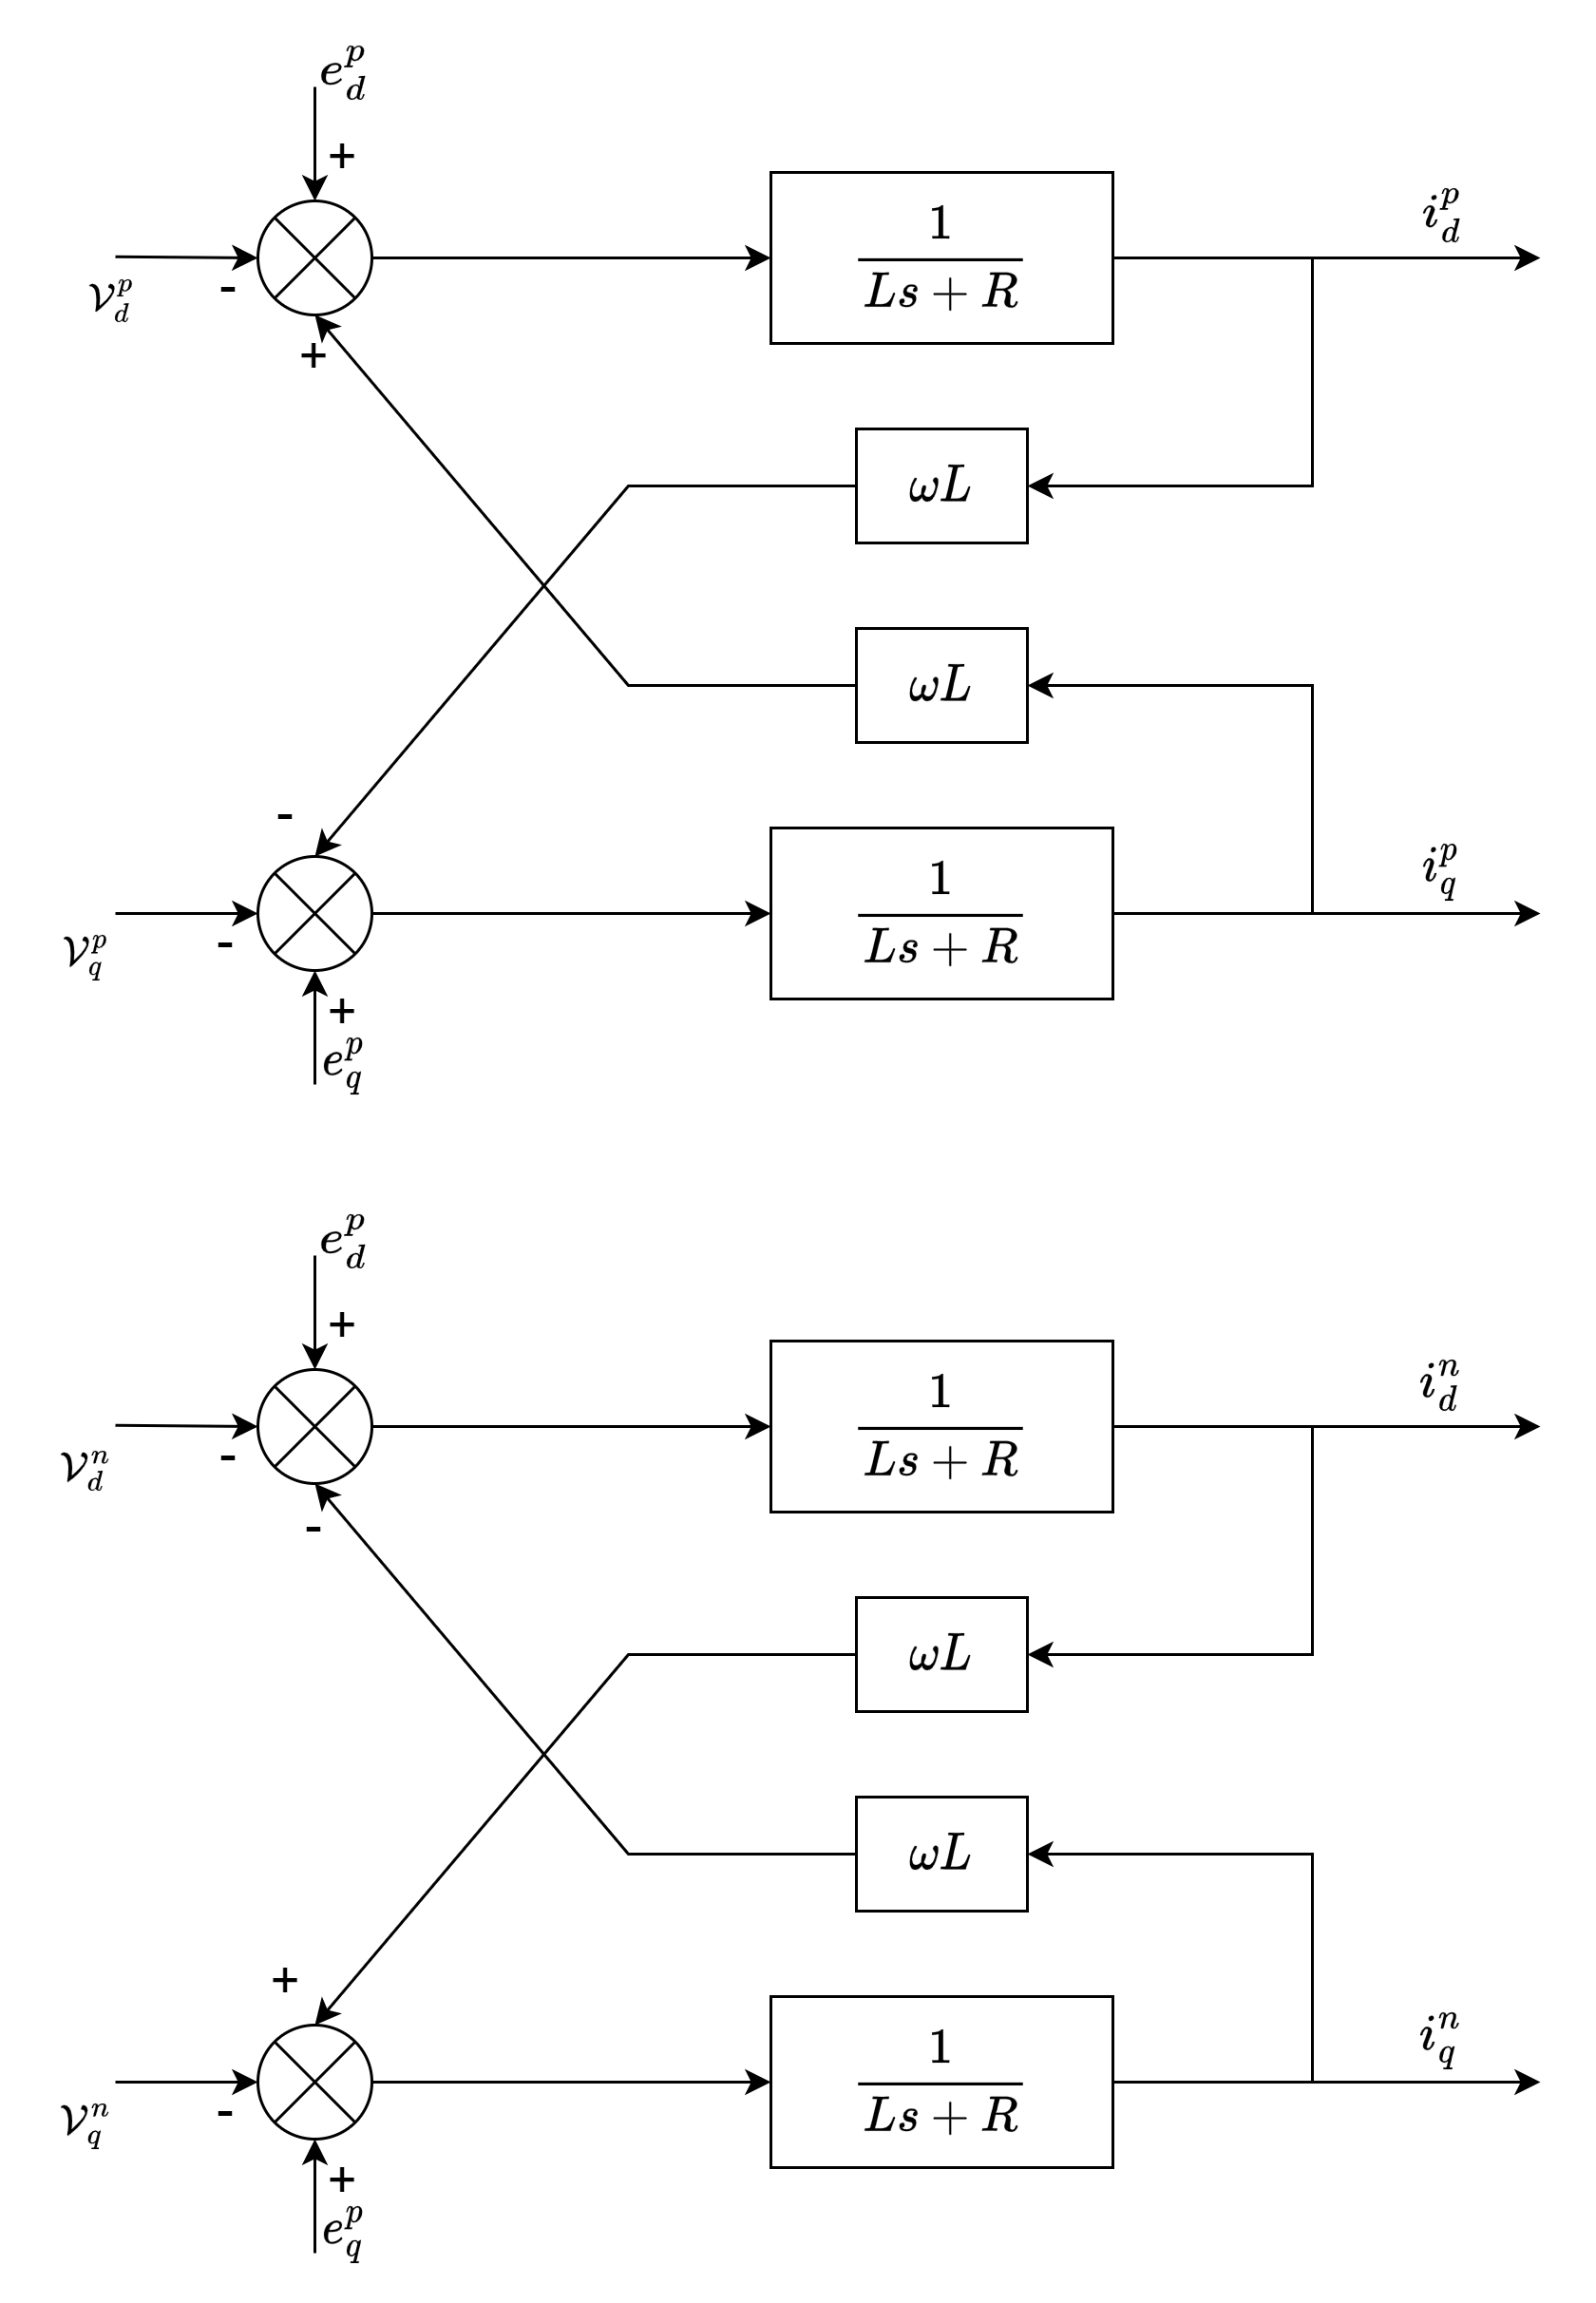
\includegraphics[scale=0.45]{img/MathematicalModel.png}
    \caption{Mathematical model of VSR in d-q coordinates}
    \label{fig:mathematical_model}
\end{figure}
\section{Effect of unbalanced grid voltage}
The performance of three phase active rectifer is highly infuenced by the grid voltage conditions.
The unbalanced grid voltage can lead to asymmetrical current fow in the system, which can
cause overheating of the components. Also the negative sequence component causes an even
harmonic ripple in the DC link voltage, which can lead to higher harmonic distortion in the
input current.\par
Under unbalanced grid conditions the input apparent power of the system can be expressed as
follows:
\begin{equation}
    S(t) = E_a I_a + E_b I_b + E_c I_c = P(t) + jQ(t)
    \label{eq:apparent_power_equation}
\end{equation}
Applying the Clarke transformation to equation[\ref{eq:apparent_power_equation}] gives the apparent
power in $\alpha\beta$ coordinates as:
\begin{equation}
    S(t) = \frac{3}{2}(E_{\alpha} + jE_{\beta})(i_{\alpha} + ji_{\beta})^{*}
\end{equation}
Based on the phasor diagram in figure[\ref{fig:symmetricalDecomposition}], the current vector $\vec{i_{s}}$ can be expressed as vector sum of
$\alpha$ and $\beta$ component currents. Then by inverse Park transformation, $\vec{i_{s}}$ is expressed:
\begin{equation}
    \begin{split}
            \vec{i_{s}} &= i_{\alpha}^{p} + ji_{\beta}^{p} + i_{\alpha}^{n} + ji_{\beta}^{n} 
    \end{split}
\end{equation}
\section{Space vector modulation}
\section{Model predictive control}
\section{Per-Unit model representation}